	{\centering\chapter{数值实验}}
	
	本科生毕业设计(论文)的正文是主体部分,要着重反映自己的工作,突出新的见解,例如新思想、新观点、新规律、新研究方法、新结果等。正文可以包括:调查对象、实验和观测方法、仪器设备、材料原料、实验和观测结果、计算方法和编程原理、数据资料、经过加工整理的图表、形成的论点和导出的结论等。
	
	正文要求论点正确,推理严数据可靠,文字精练,条理分明,文字图表清晰整齐。利用别人研究成果必须附加说明。引用前人材料必须引证原著文字。在论文的行文上,要注意语句通顺,达到科技论文所必须具备的"正确、准确、明确"的要求。
	
	由于研究工作涉及的学科、选题、研究方法、工作进程、结果表达方式等有很大的差异,不对正文内容作统一硬性的规定。但是,必须实事求是,合乎逻辑,层次分明。

\begin{lemma}\label{LemmaLbeta}
	Let $\left\{ \mathbf{x}^{k}, \mathbf{y}^{k}, \mathbf{z}^{k} \right\}$ be the sequences denoted by {\tt ADMM}$_{\ell_{1}/\ell_{\infty}}$, and then we have 
	\begin{equation} 
			\mathcal{L}_{\beta} \left( \mathbf{x}^{k+1}, \mathbf{y}^{k+1}, \mathbf{z}^{k+1} \right) \leq  \left(\frac{\lambda_{\min}  \left( \mathbf{A}^{\top} \mathbf{A} \right)}{2}  +  \frac{\beta}{2} - \frac{L_f^2}{\beta} \right) \left \Vert \mathbf{y}^{k+1} - \mathbf{y}^{k} \right \Vert_{2}^{2},
	\end{equation} 
	where $L_f \triangleq \lambda_{\max} \left( \mathbf{A}^{\top} \mathbf{A} \right)$ and  $\lambda_{\min}  \left( \mathbf{A}^{\top} \mathbf{A} \right) > 0$  is the largest and non-negative smallest eigenvalue of $ \mathbf{A}^{\top} \mathbf{A}$, respectively.
\end{lemma}
	
	\section{格式要求}
	 
\begin{proposition}\label{LemmaLbeta1}
	Let $\left\{ \mathbf{x}^{k}, \mathbf{y}^{k}, \mathbf{z}^{k} \right\}$ be the sequences denoted by {\tt ADMM}$_{\ell_{1}/\ell_{\infty}}$, and then we have 
	\begin{equation} 
			\mathcal{L}_{\beta} \left( \mathbf{x}^{k+1}, \mathbf{y}^{k+1}, \mathbf{z}^{k+1} \right) \leq  \left(\frac{\lambda_{\min}  \left( \mathbf{A}^{\top} \mathbf{A} \right)}{2}  +  \frac{\beta}{2} - \frac{L_f^2}{\beta} \right) \left \Vert \mathbf{y}^{k+1} - \mathbf{y}^{k} \right \Vert_{2}^{2},
	\end{equation} 
	where $L_f \triangleq \lambda_{\max} \left( \mathbf{A}^{\top} \mathbf{A} \right)$ and  $\lambda_{\min}  \left( \mathbf{A}^{\top} \mathbf{A} \right) > 0$  is the largest and non-negative smallest eigenvalue of $ \mathbf{A}^{\top} \mathbf{A}$, respectively.
\end{proposition}

	\section{图、表格和公式要求}
	
	文中的图、表、附注、公式一律采用阿拉伯数字分章编号。如:图2-5,表3-2,等。
	
	\subsection{图格式要求}
	
	插图须精心制作,线条清晰、美观,不得徒手画图,必须按国家规定标准或工程要求用计算机绘制。插图应与正文呼应,切忌与文字表述重复。不得插入与正文无关的图表或照片。插图应有图题,图序及图名居中置于图的正下方,图中的术语、符号、单位等应同文字表述一致。插图为嵌入型居中排列。图中字体及大小根据实际情况自行调整。
	
	\begin{figure}[h]
%		\bicaption{中文图名}{英文图名}\label{tab:fig1} % 放在这里,标注在表上面
		\centering
		\subfloat[\zihao{5}图a标题]{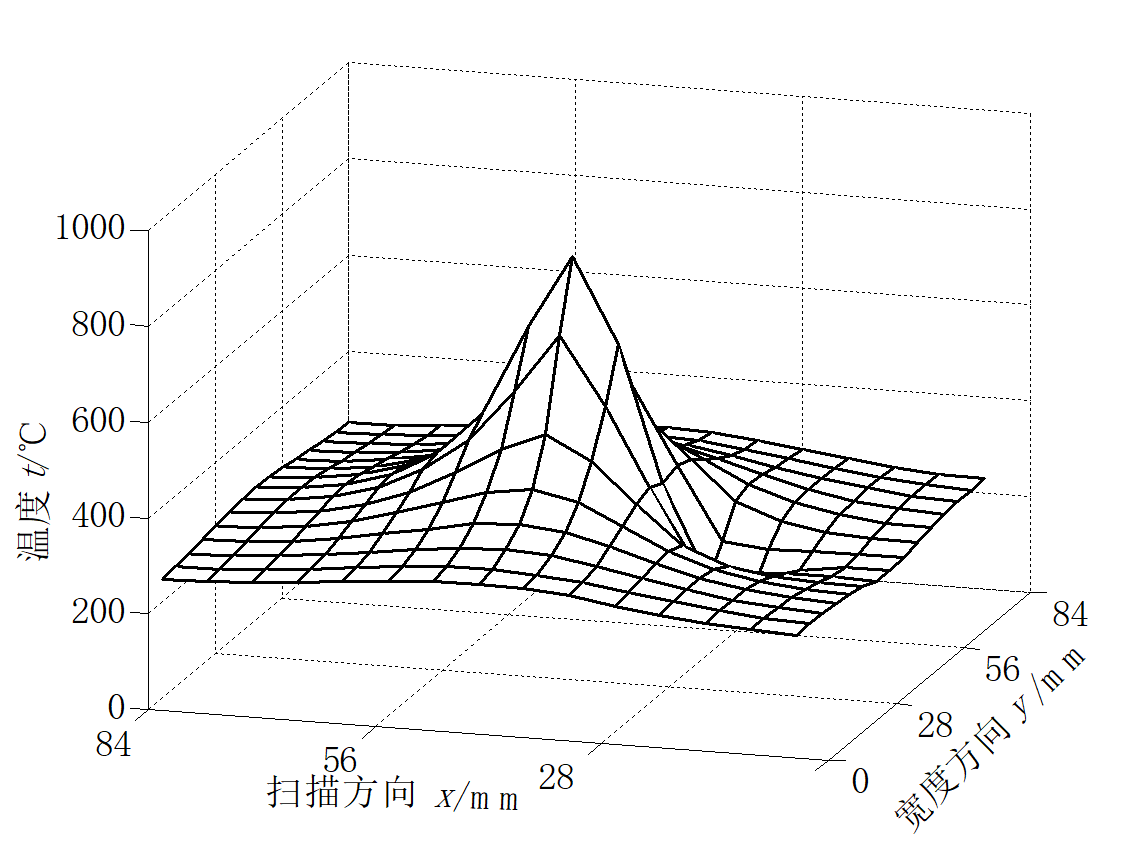
\includegraphics[width=0.4\textwidth]{fig21a.png}\label{fig1}}\hspace{30pt}
		\subfloat[图b标题]{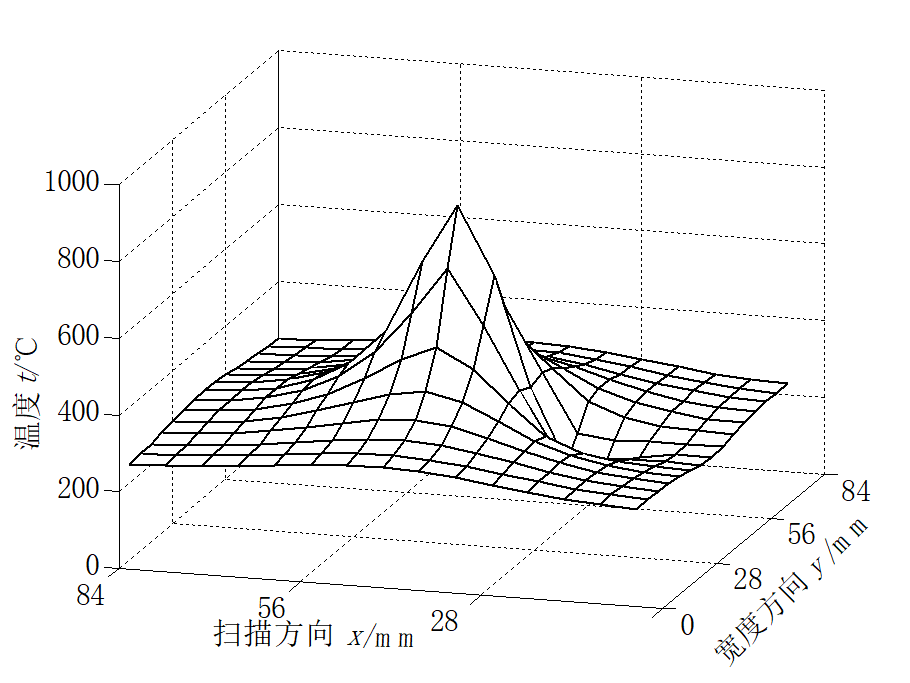
\includegraphics[width=0.4\textwidth]{fig21b.png}}
		\bicaption{中文图名}{英文图名}\label{tab:fig1} % 放在这里,标注在表下面
	\end{figure}
	
	\subsection{表格式要求}
	
	表中参数应标明量和单位的符号。表中字体及大小根据实际情况自行调整。行间距为单倍行距。表序号及表名称置于表的上方。
	
	表名称:正文中的表要有中文名称,表的中文名称为5号宋体字,不加粗,居中并位于表上;
	
	表尺寸:表尽量以一页的页面为限,一旦超限要加续表;
	
	表位置:表居中排列;
	
	表格式:三线表。三线表的组成要素包括:表序、表题、项目栏、表体、表注。三线表通常只有3条线,即顶线、底线和栏目线。其中顶线和底线为粗线,栏目线为细线。如下表:
	
	\begin{table}[!ht]
%		\bicaption{中文图名}{英文图名}\label{tab:lable} % 放在这里,标注在表上面
		\begin{tabular*}{\hsize}{@{}@{\extracolsep{\fill}}lllllllllllll@{}}
			\toprule
			$p_{t}$  &21  &22  &20  &15  &10  &8   &5   &10  &18  &10  &14  &18\\
			\midrule
			$c_{t}$  &5   &13  &10  &10  &10  &10  &10  &10  &10  &10  &10  &10\\
			$h_{t}$  &10  &5   &5   &5   &5   &5   &5   &5   &5   &5   &5   &5 \\
			$s_{t}$  &100 &100 &100 &100 &100 &100 &100 &100 &100 &100 &100 &100\\
			$d_{t}$  &30  &45  &50  &55  &45  &55  &90  &80  &90  &65  &80  &70 \\
			\bottomrule
		\end{tabular*}
		\bicaption{中文图名}{英文图名}\label{tab:lable} % 放在这里,标注在表下面
	\end{table}
	
	\subsection{公式}
	 